\chapter{Dependencies of \rmue}
\label{app:rmue}
\begin{figure}[htbp]
\centering
\begin{minipage}[t]{0.49\textwidth}
  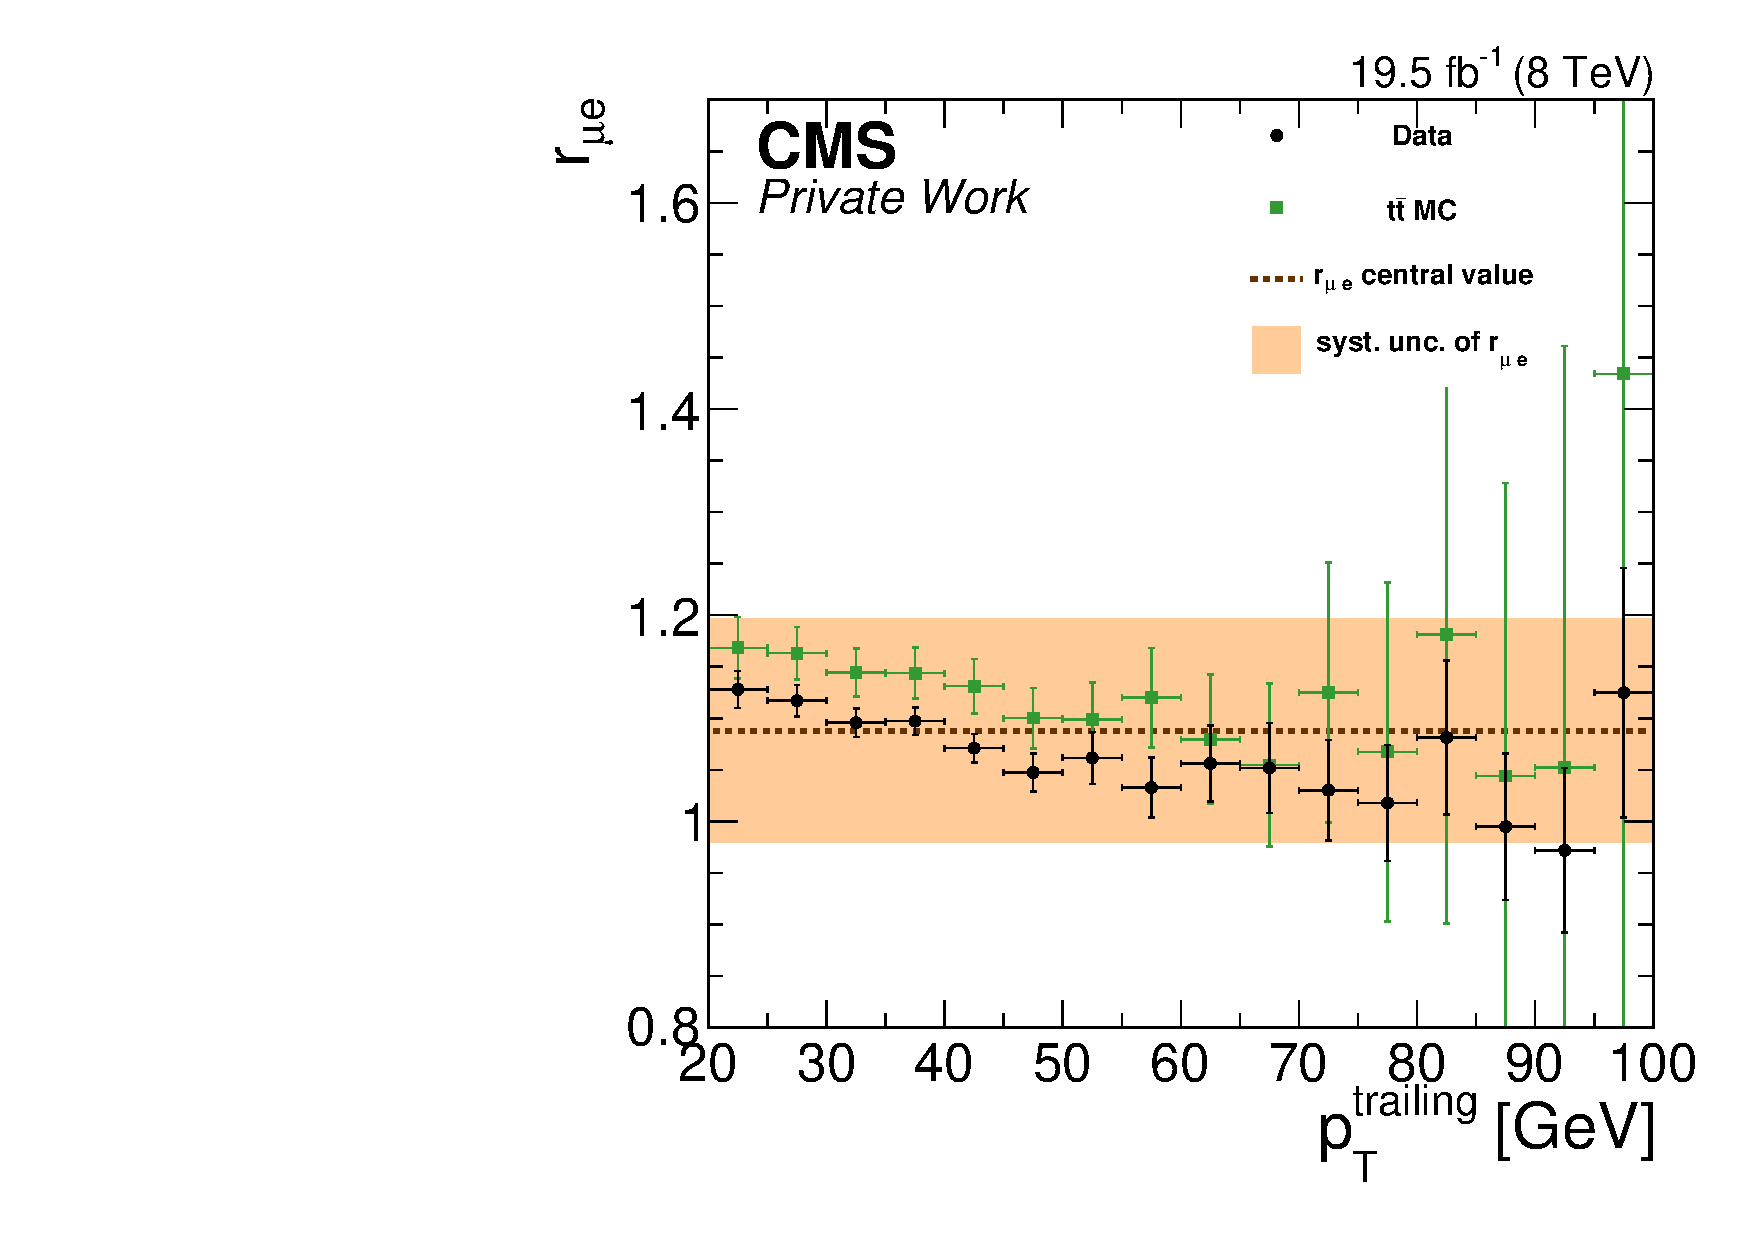
\includegraphics[width=\textwidth]{plots/BG/rmue/rMuE_ZPeakControlCentral_Full2012_TrailingPt_leadingPt30.pdf}
\end{minipage}
\begin{minipage}[t]{0.49\textwidth}
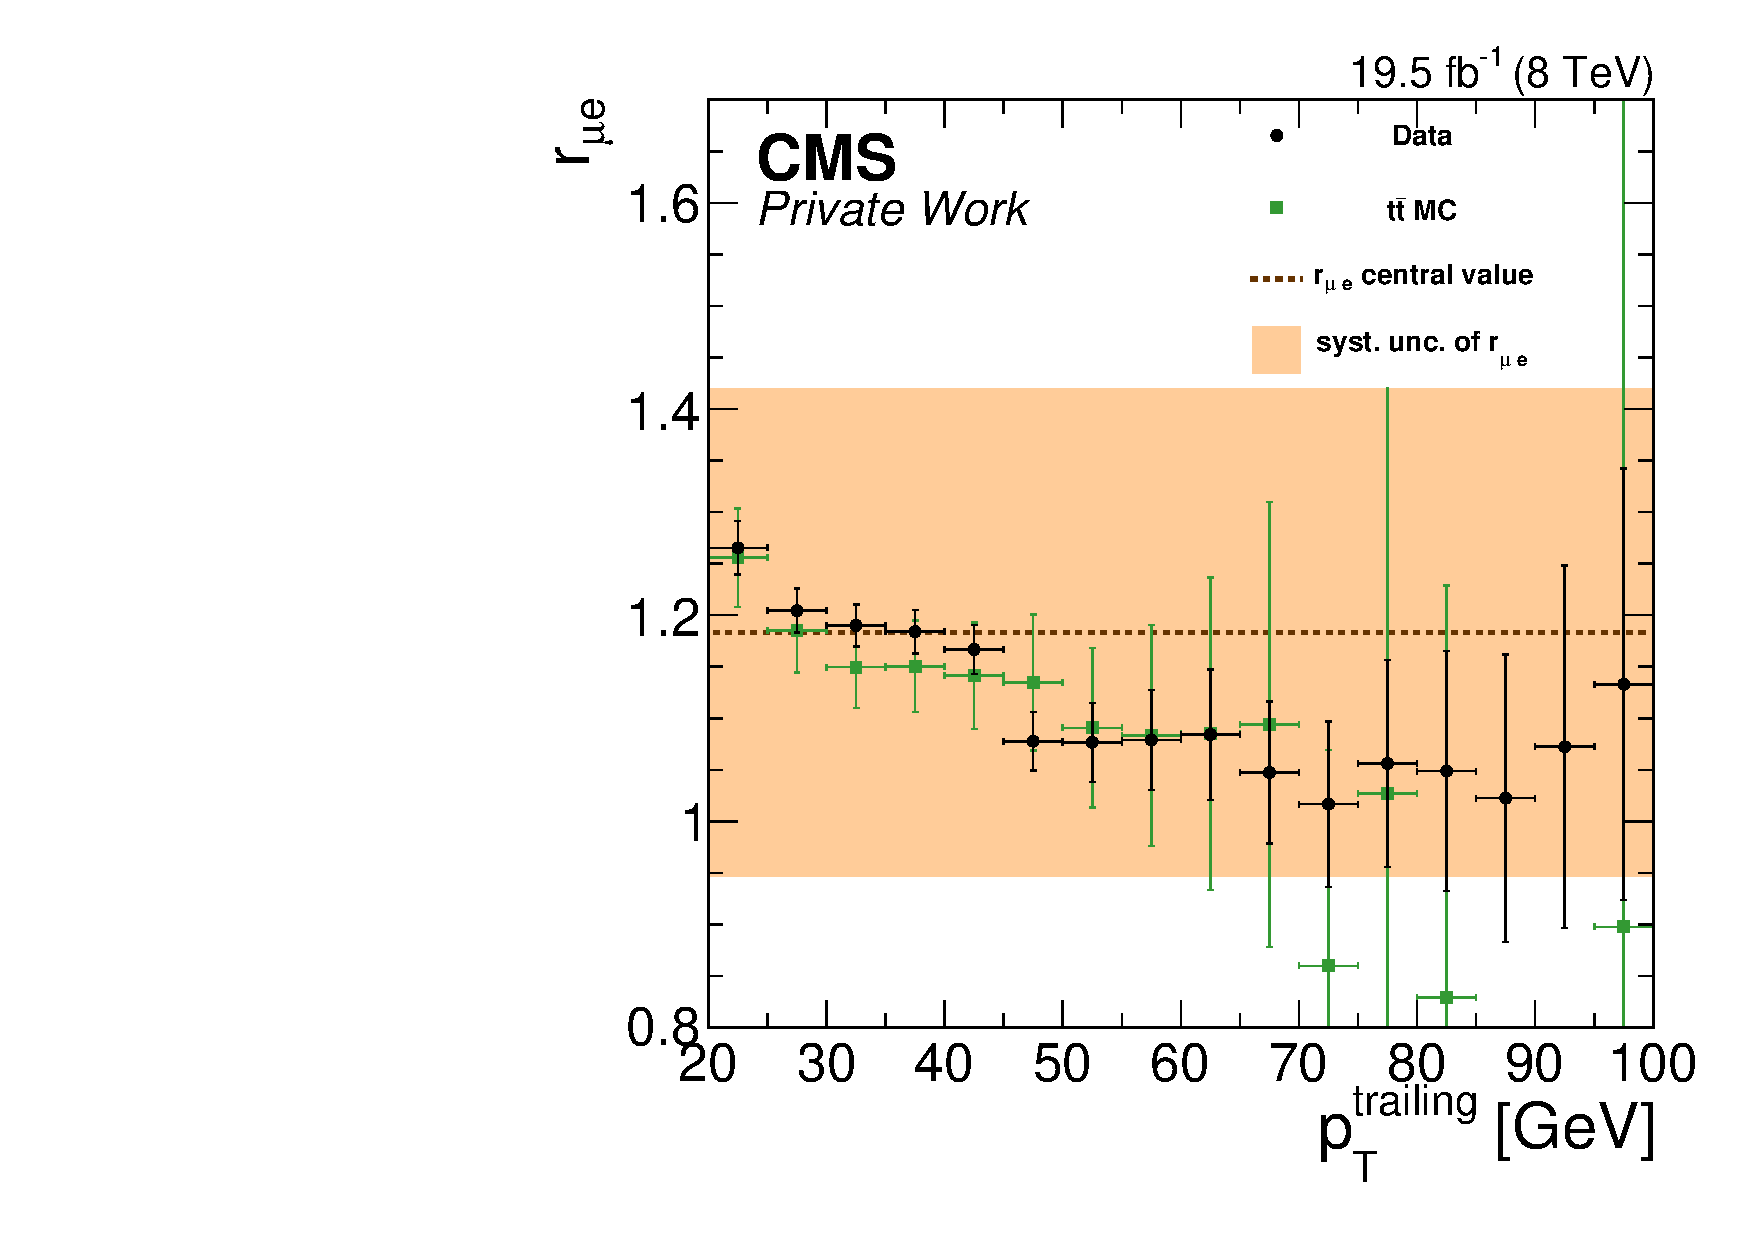
\includegraphics[width=\textwidth]{plots/BG/rmue/rMuE_ZPeakControlForward_Full2012_TrailingPt_leadingPt30.pdf}
\end{minipage}
\begin{minipage}[t]{0.49\textwidth}
  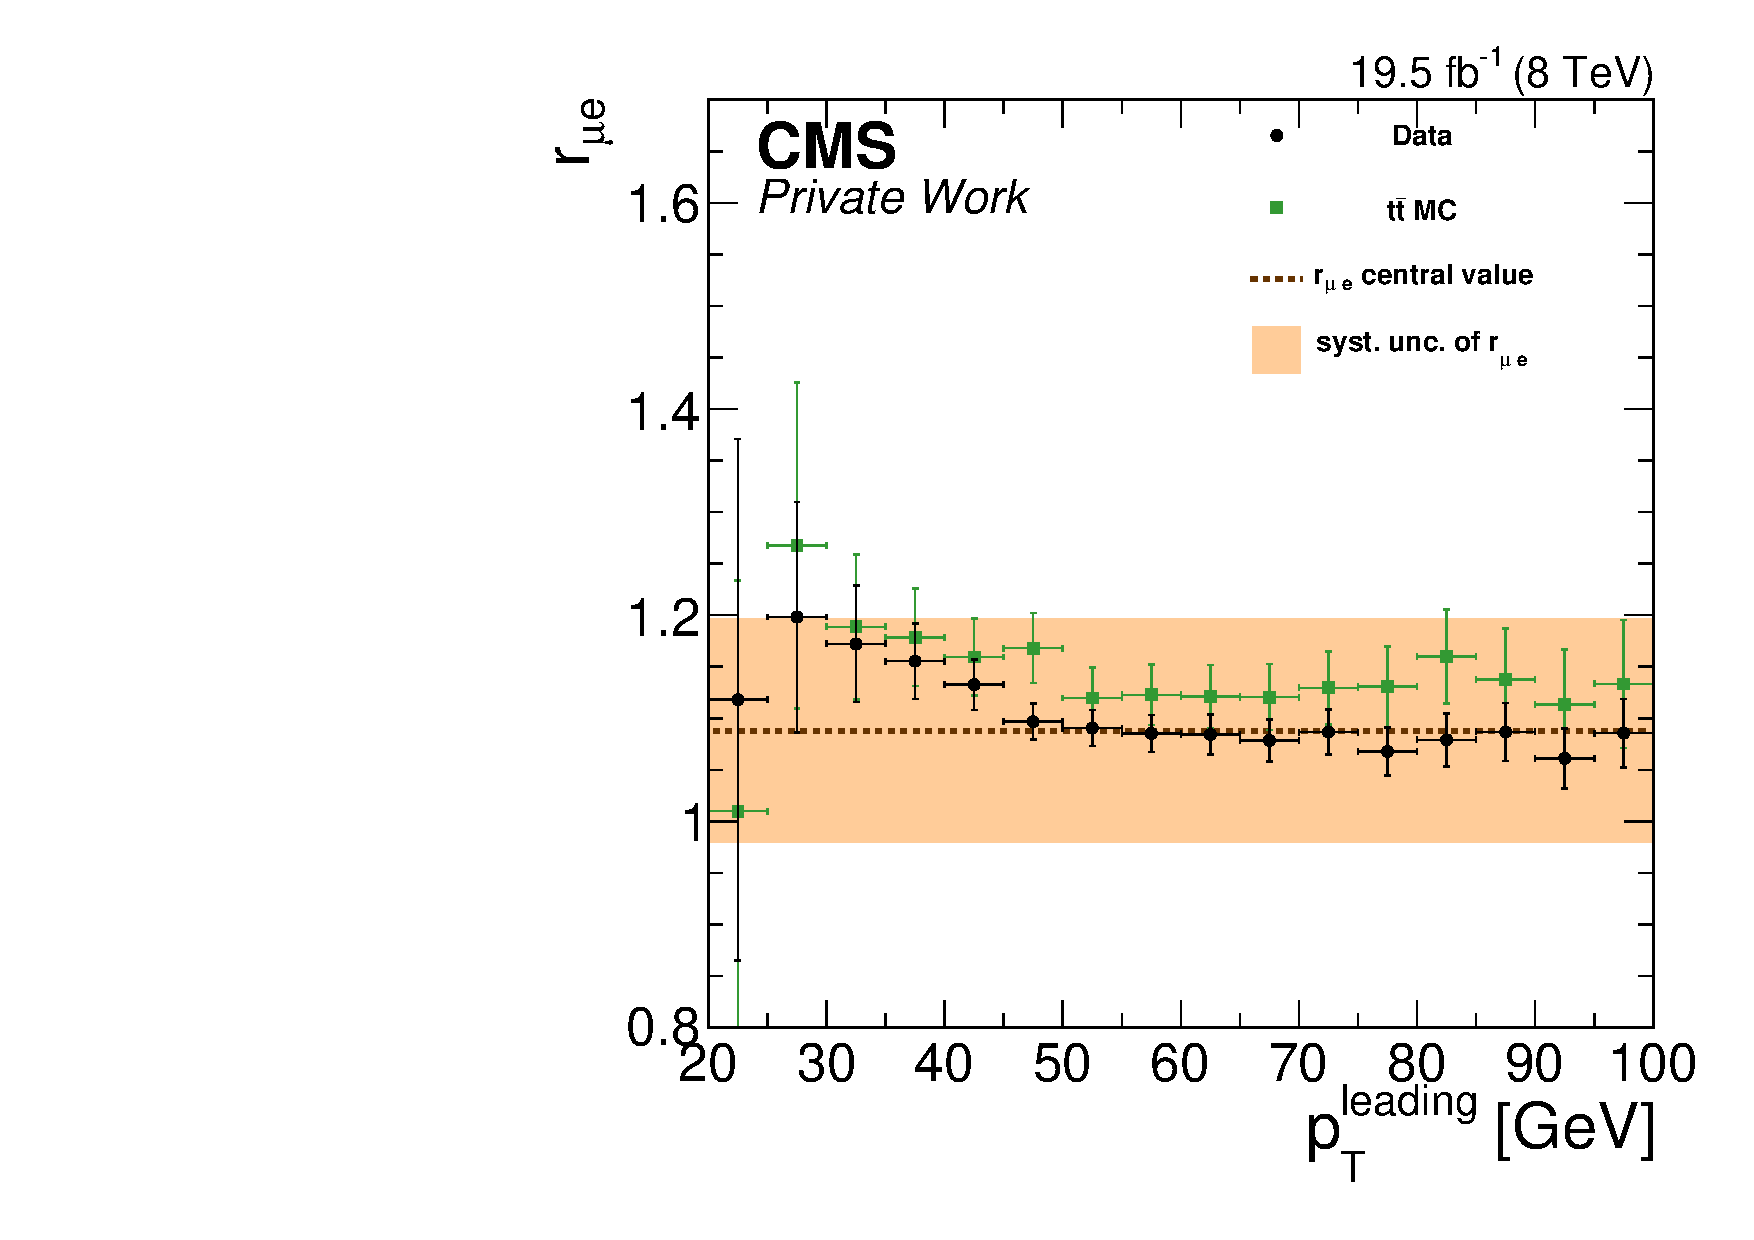
\includegraphics[width=\textwidth]{plots/BG/rmue/rMuE_ZPeakControlCentral_Full2012_LeadingPt_trailingPt20.pdf}
\end{minipage}
\begin{minipage}[t]{0.49\textwidth}
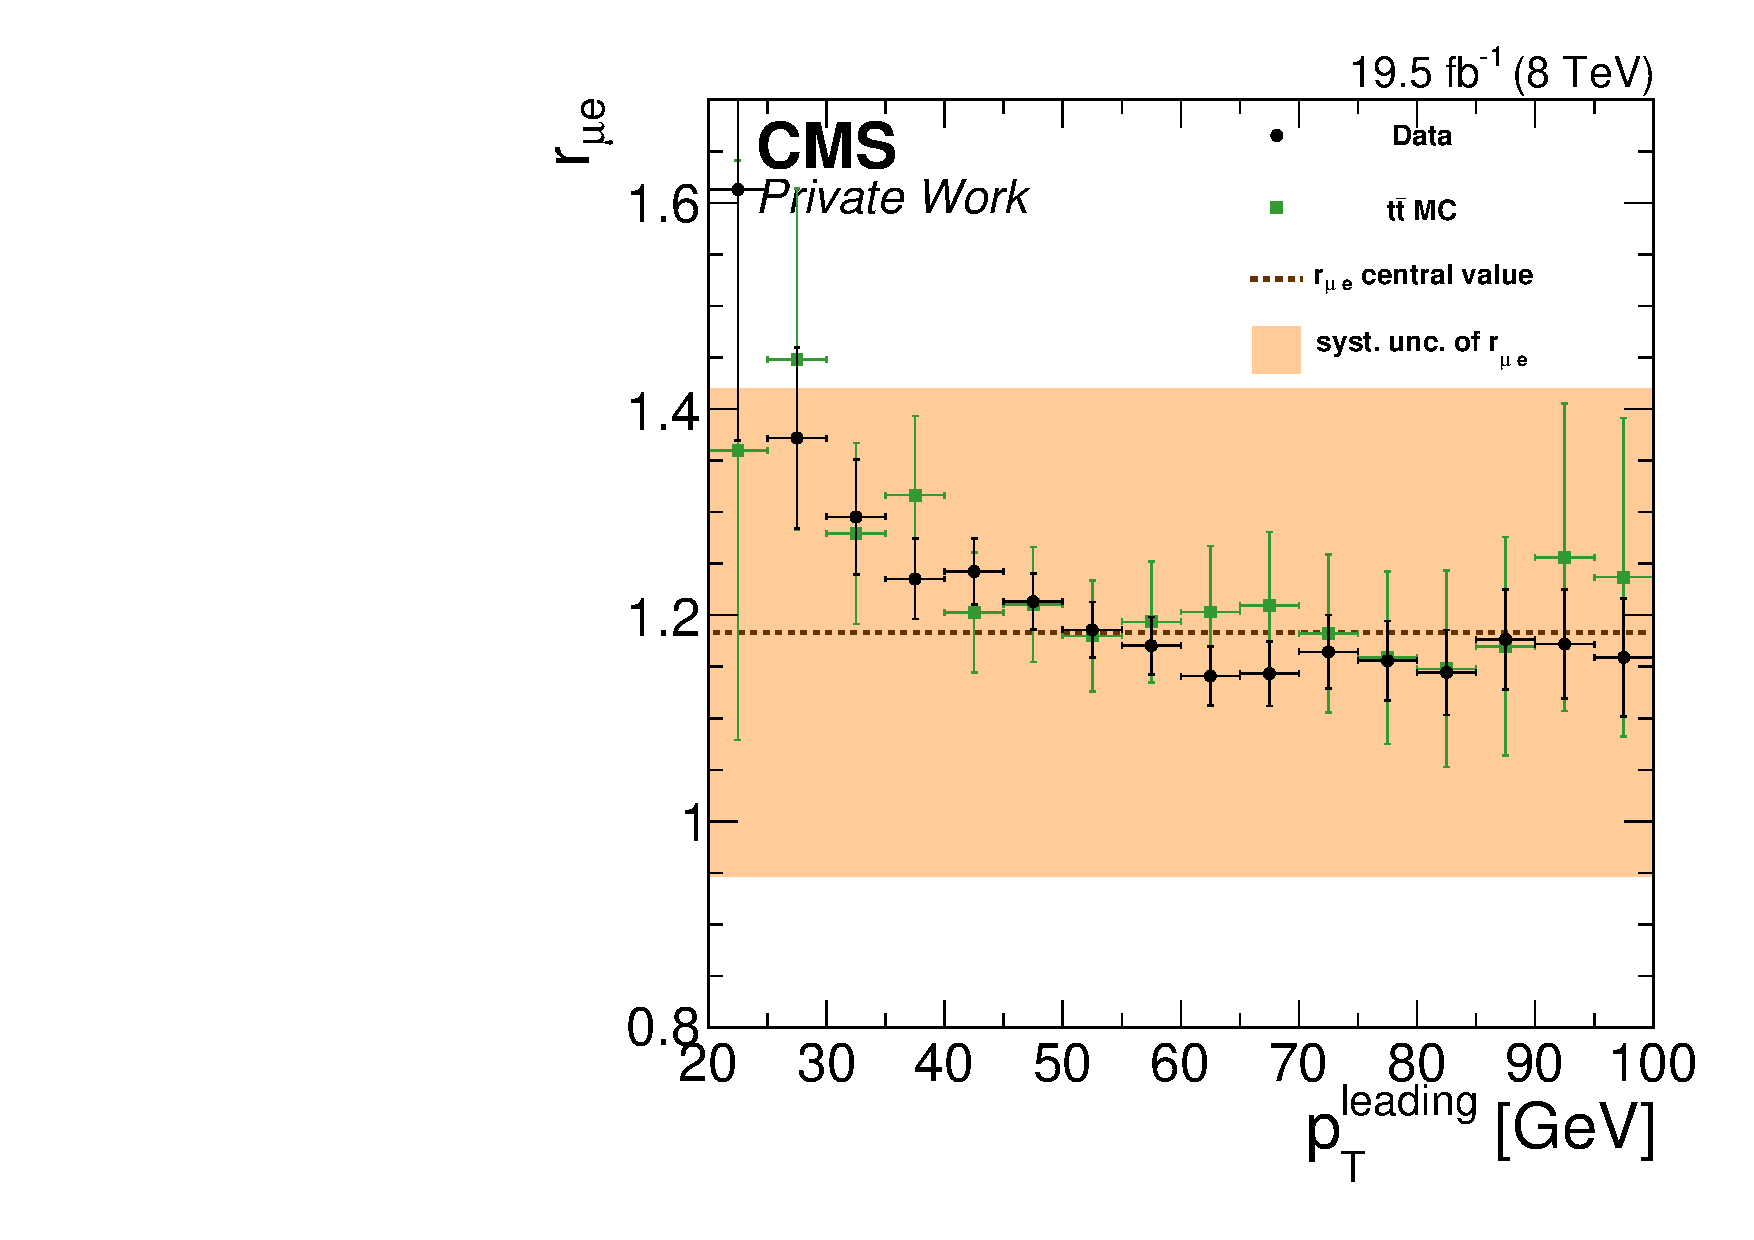
\includegraphics[width=\textwidth]{plots/BG/rmue/rMuE_ZPeakControlForward_Full2012_LeadingPt_trailingPt20.pdf}
\end{minipage}

\caption{Dependencies of \rmue on the \pt of the trailing (top) and the leading (bottom) lepton for the central (left) and forward (right) lepton selection. The results on data are shown in black while $t\bar{t}$ simulation is shown in green. The central value is shown as a brown dashed line while the systematic uncertainty is shown as an orange band.}
\label{fig:rmueDependenciesApp1}
\end{figure} 

\begin{figure}[htbp]
\centering
\begin{minipage}[t]{0.49\textwidth}
  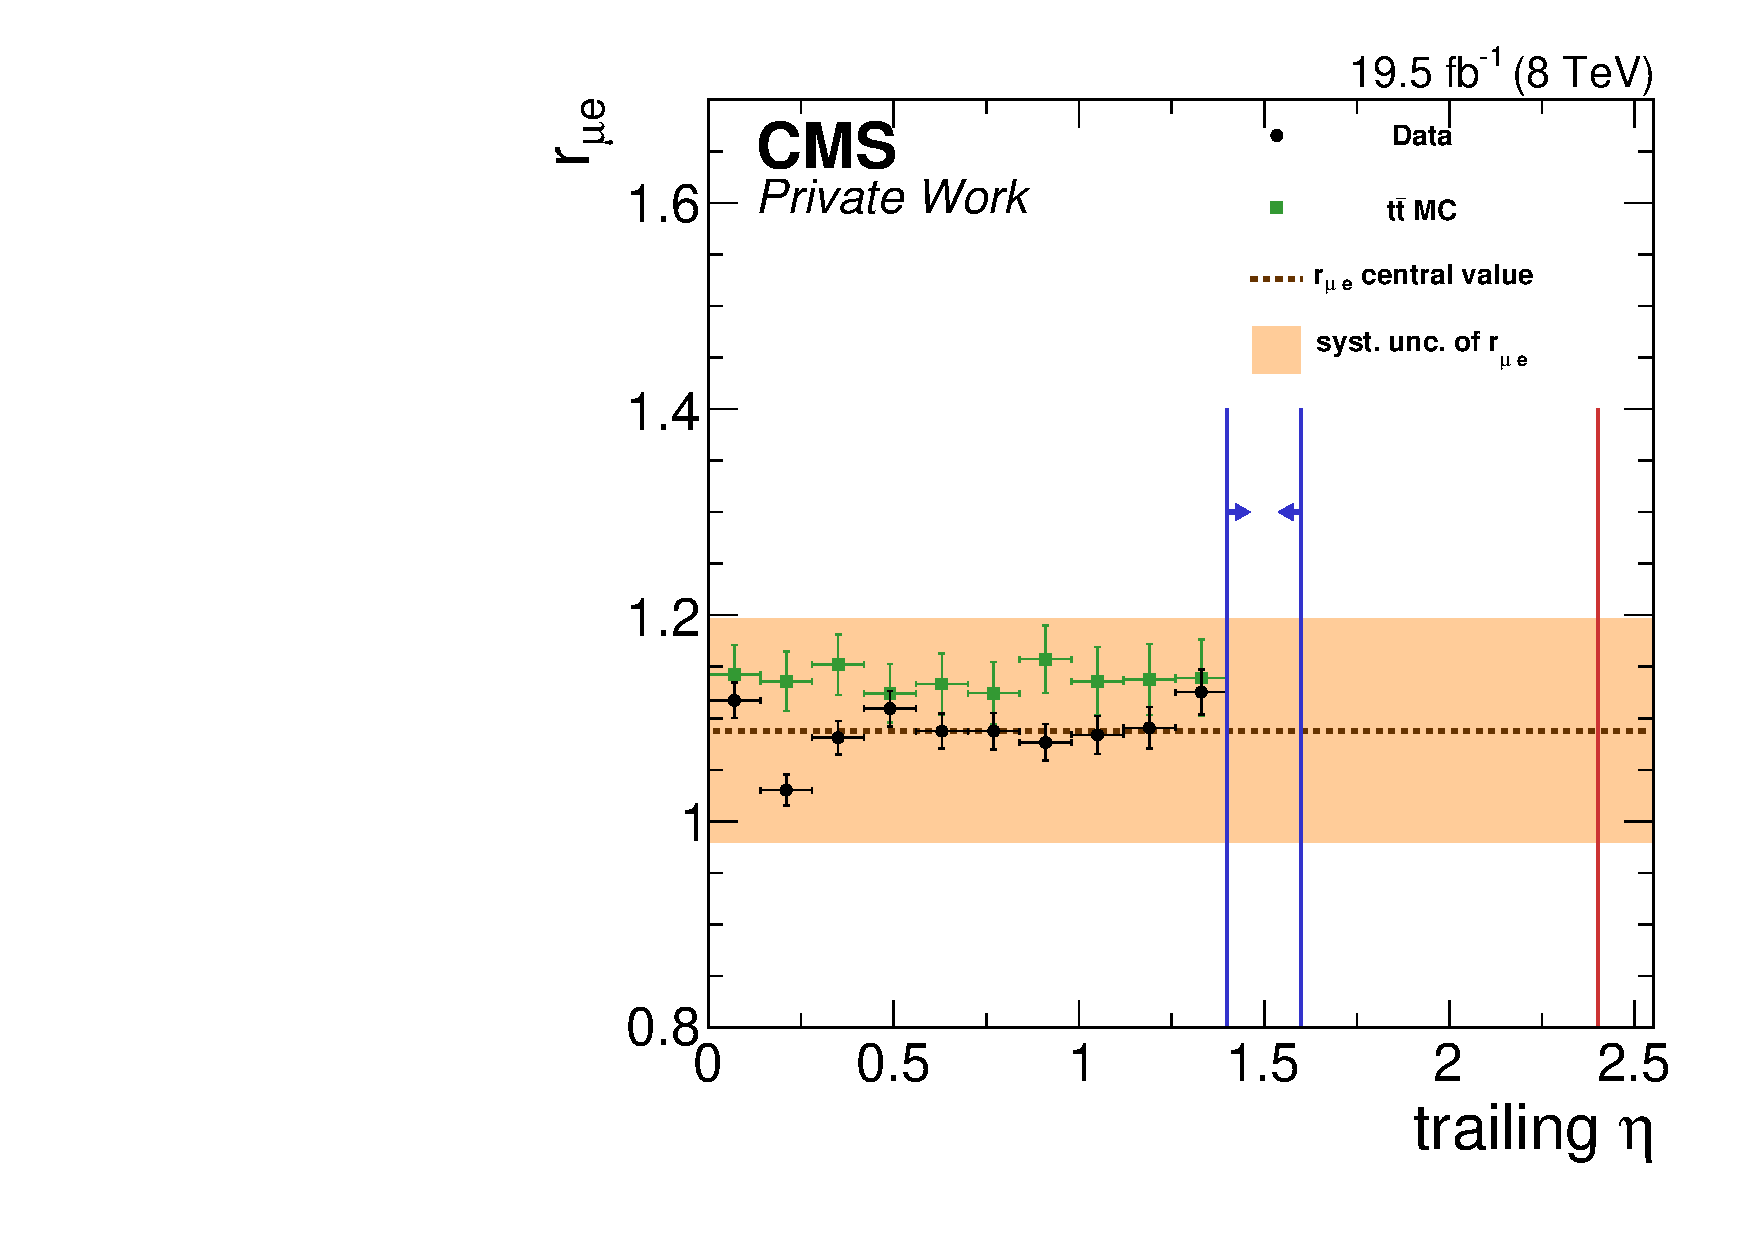
\includegraphics[width=\textwidth]{plots/BG/rmue/rMuE_ZPeakControlCentral_Full2012_TrailingEta_None.pdf}
\end{minipage}
\begin{minipage}[t]{0.49\textwidth}
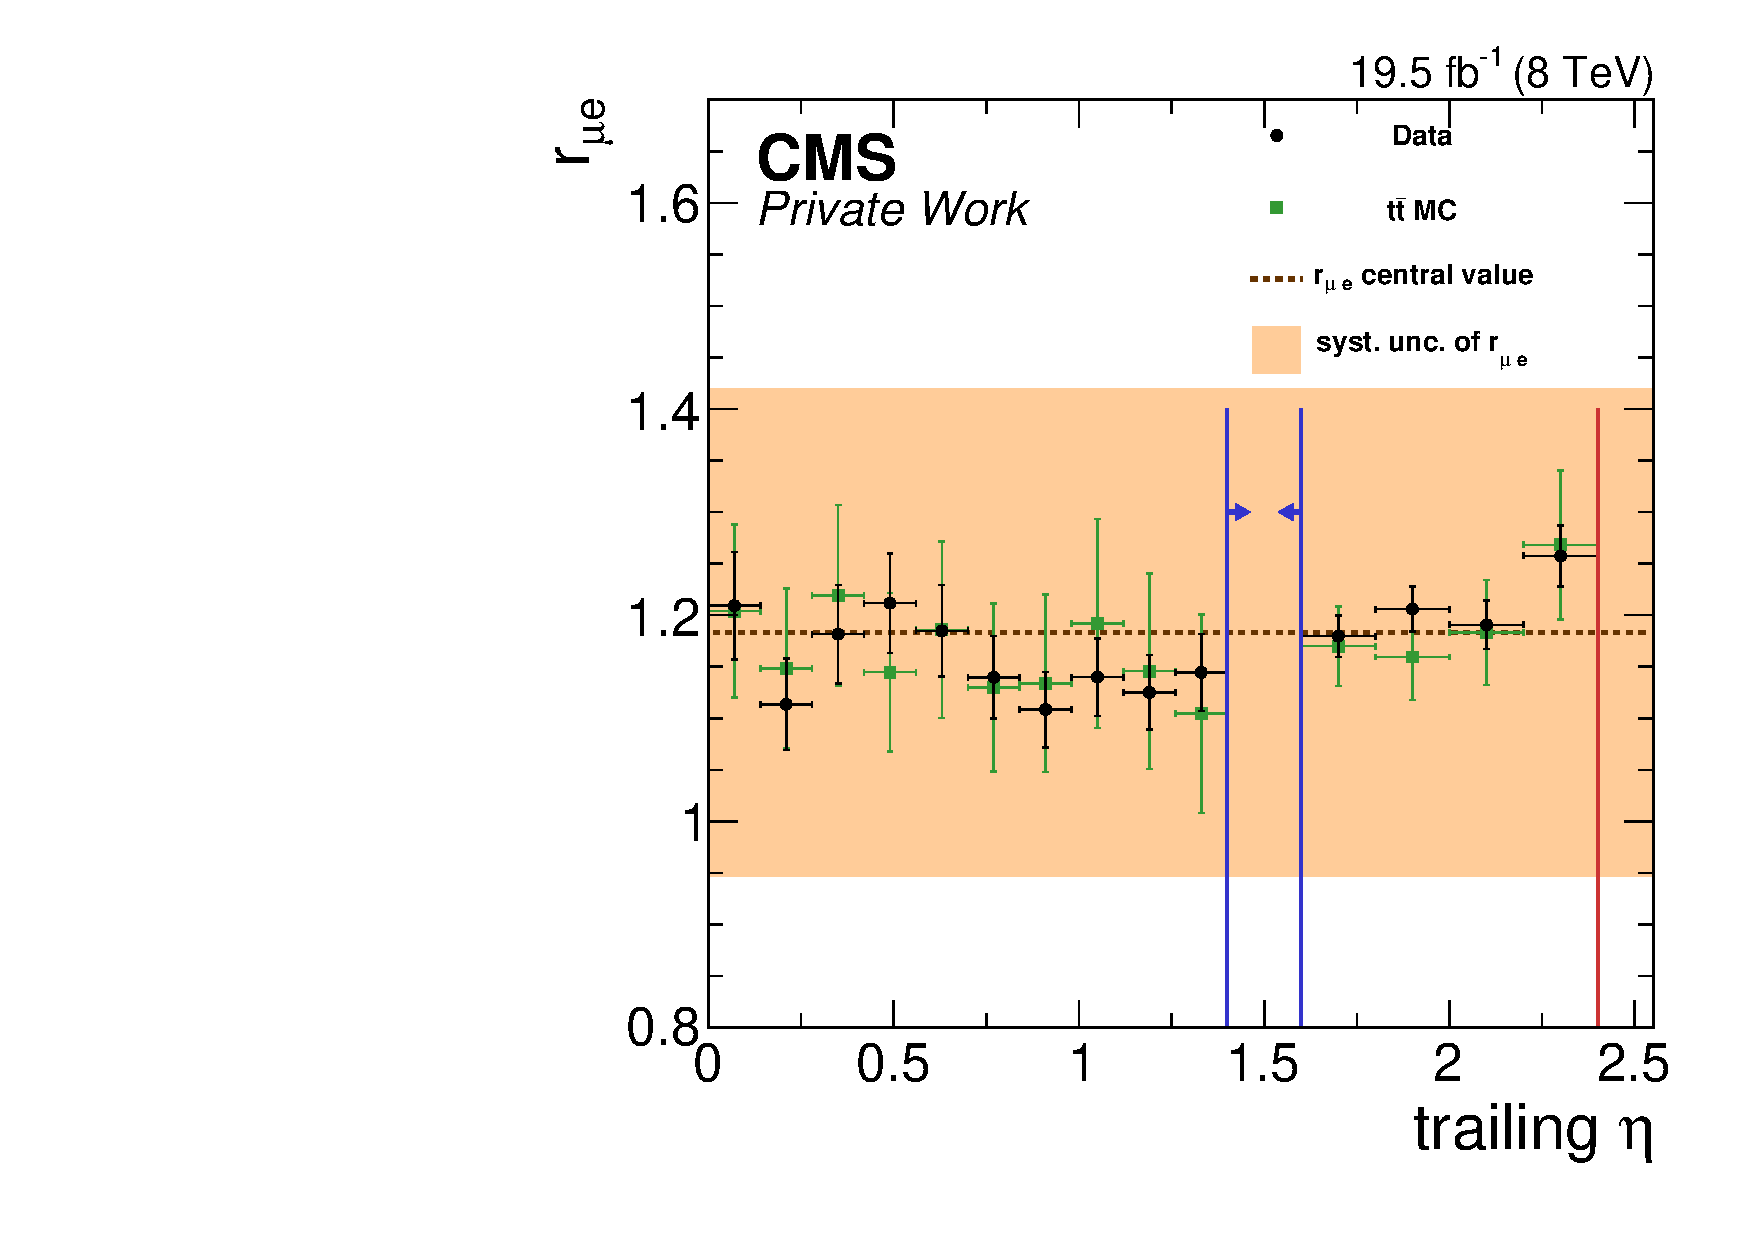
\includegraphics[width=\textwidth]{plots/BG/rmue/rMuE_ZPeakControlForward_Full2012_TrailingEta_None.pdf}
\end{minipage}
\begin{minipage}[t]{0.49\textwidth}
  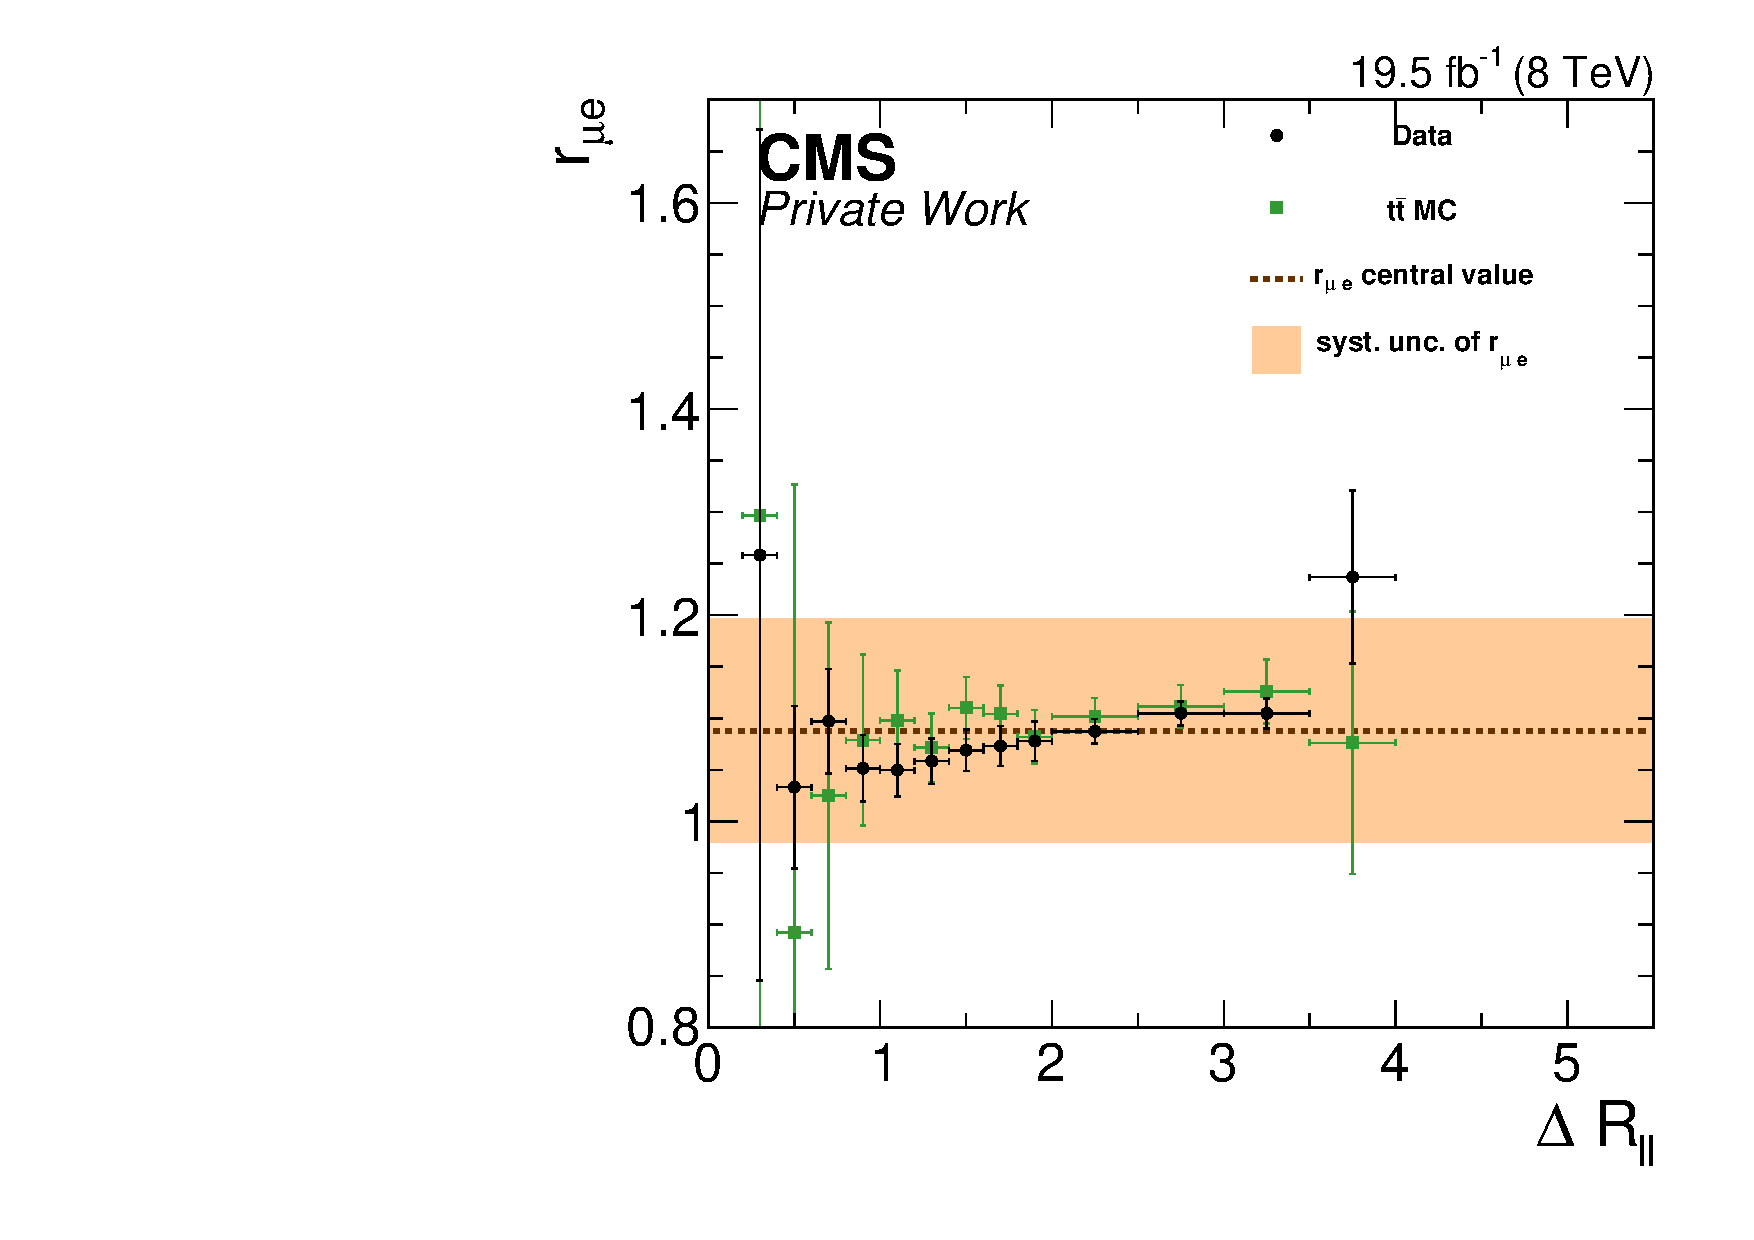
\includegraphics[width=\textwidth]{plots/BG/rmue/rMuE_ZPeakControlCentral_Full2012_DeltaR_None.pdf}
\end{minipage}
\begin{minipage}[t]{0.49\textwidth}
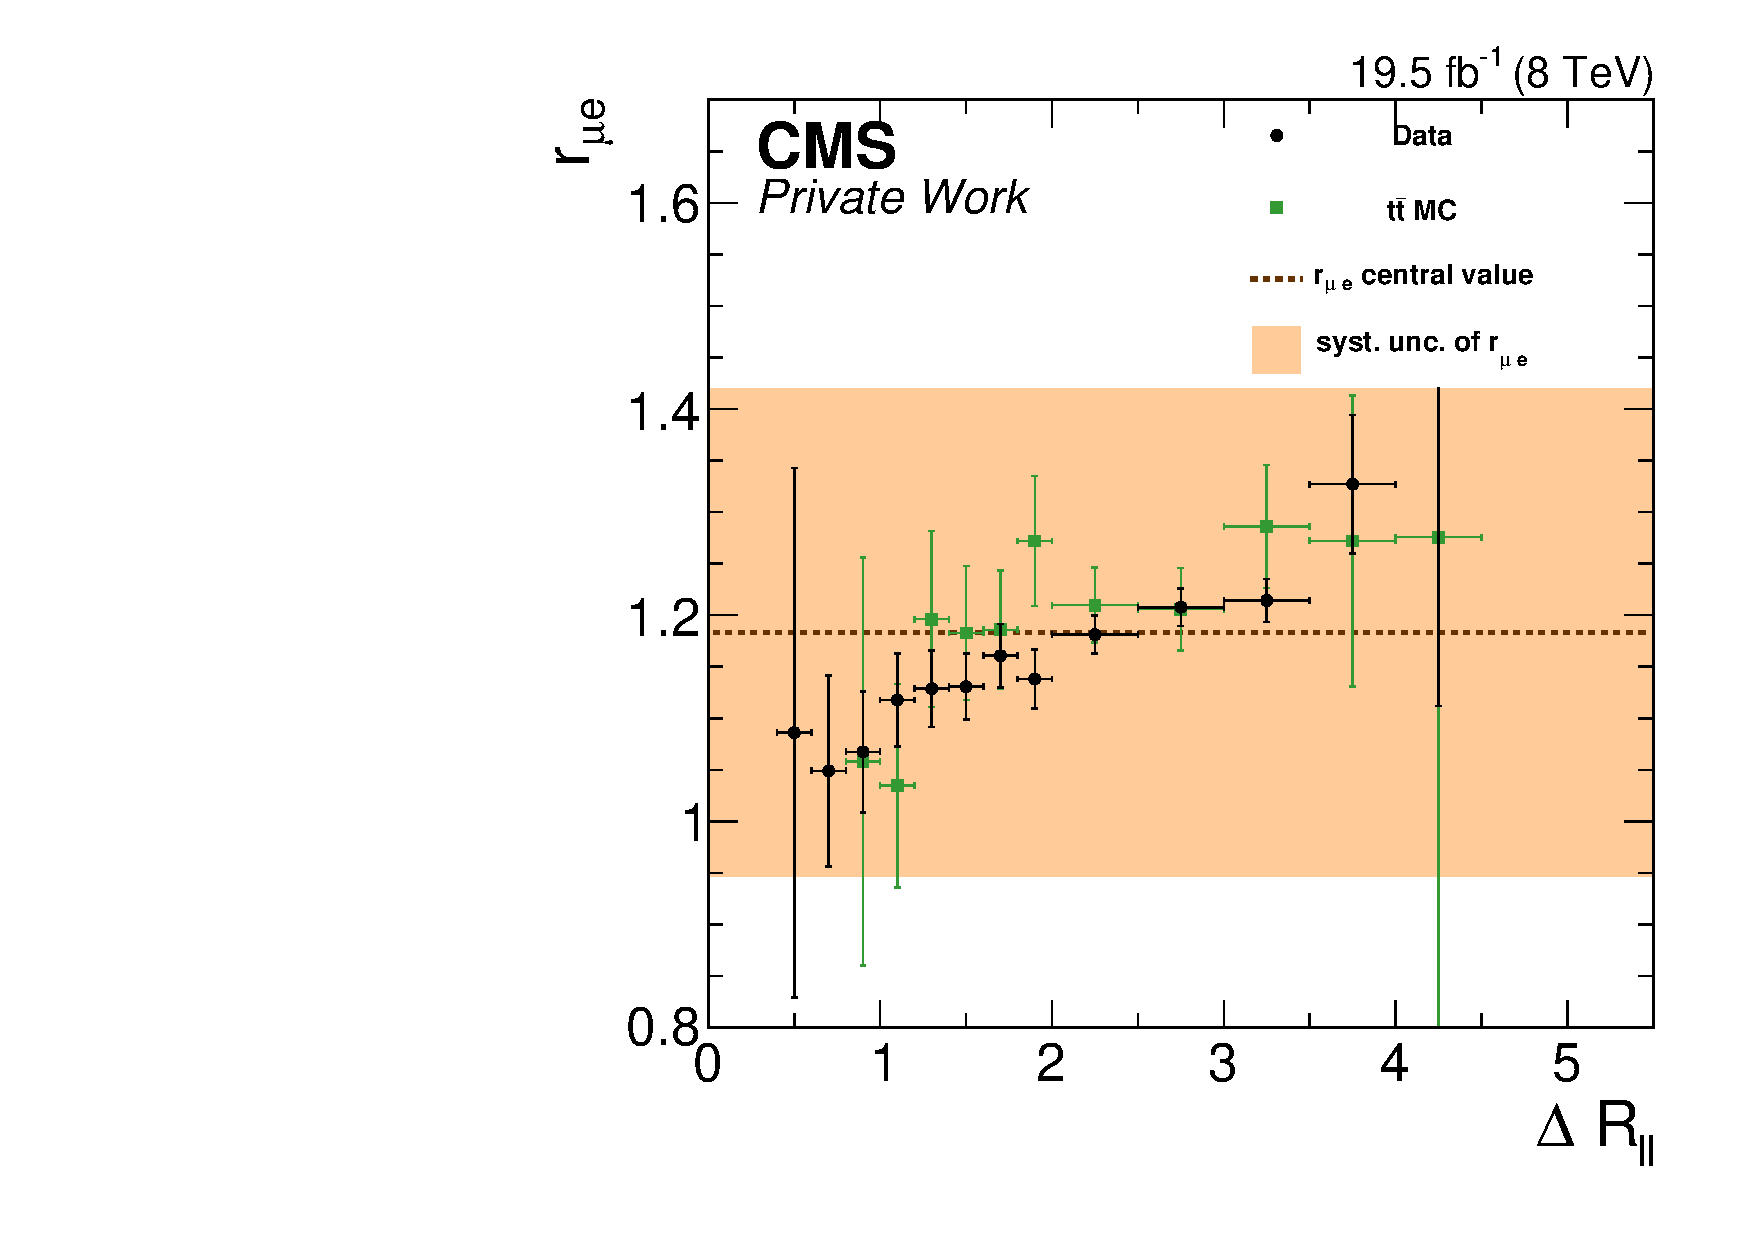
\includegraphics[width=\textwidth]{plots/BG/rmue/rMuE_ZPeakControlForward_Full2012_DeltaR_None.pdf}
\end{minipage}
\caption{Dependencies of \rmue on the $|\eta|$ of the trailing lepton (top) and  $\Delta R(\ell\ell)$ (bottom) for the central (left) and forward (right) lepton selection. The results on data are shown in black while $t\bar{t}$ simulation is shown in green. The central value is shown as a brown dashed line while the systematic uncertainty is shown as an orange band.}
\label{fig:rmueDependenciesApp2}
\end{figure} 


\begin{figure}[t]
\centering
\begin{minipage}[t]{0.49\textwidth}
  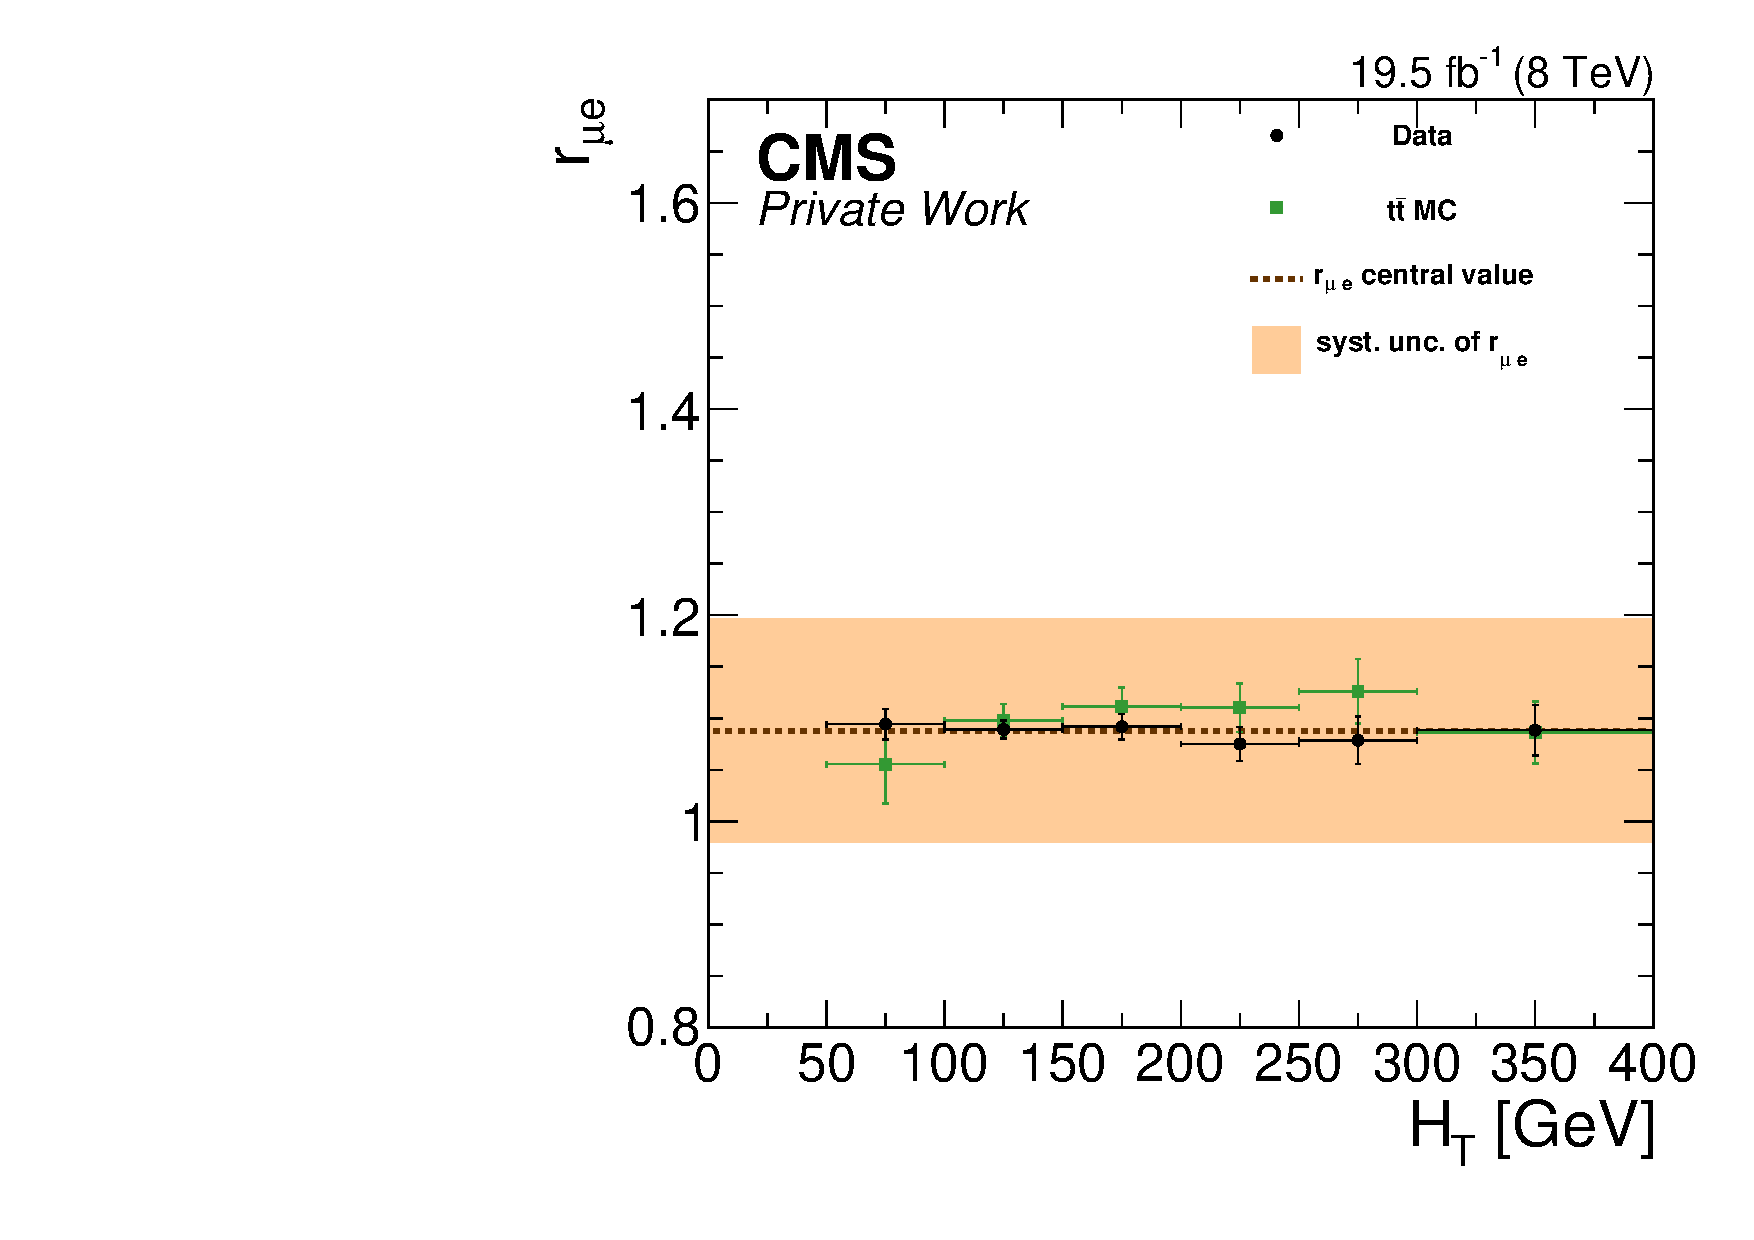
\includegraphics[width=\textwidth]{plots/BG/rmue/rMuE_ZPeakControlCentral_Full2012_HT_None.pdf}
\end{minipage}
\begin{minipage}[t]{0.49\textwidth}
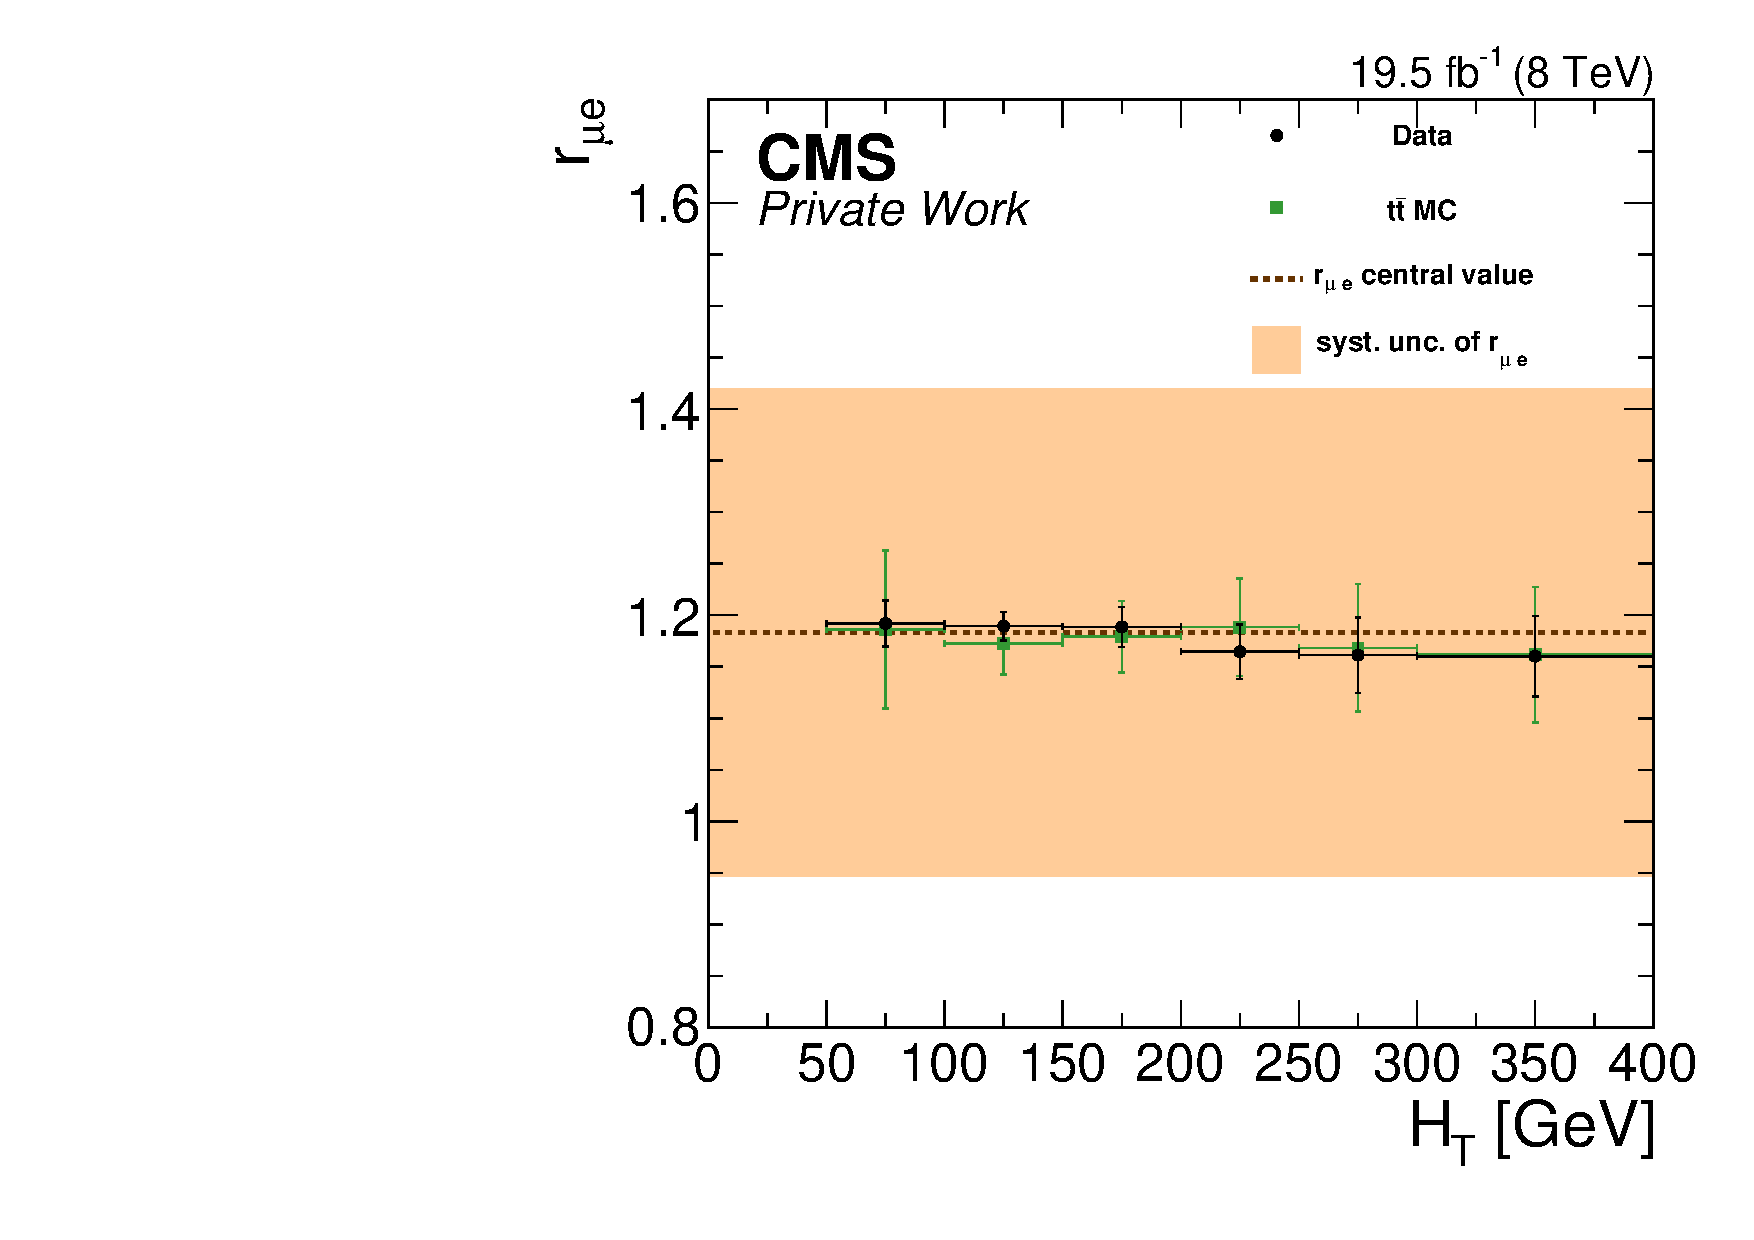
\includegraphics[width=\textwidth]{plots/BG/rmue/rMuE_ZPeakControlForward_Full2012_HT_None.pdf}
\end{minipage}
\begin{minipage}[t]{0.49\textwidth}
  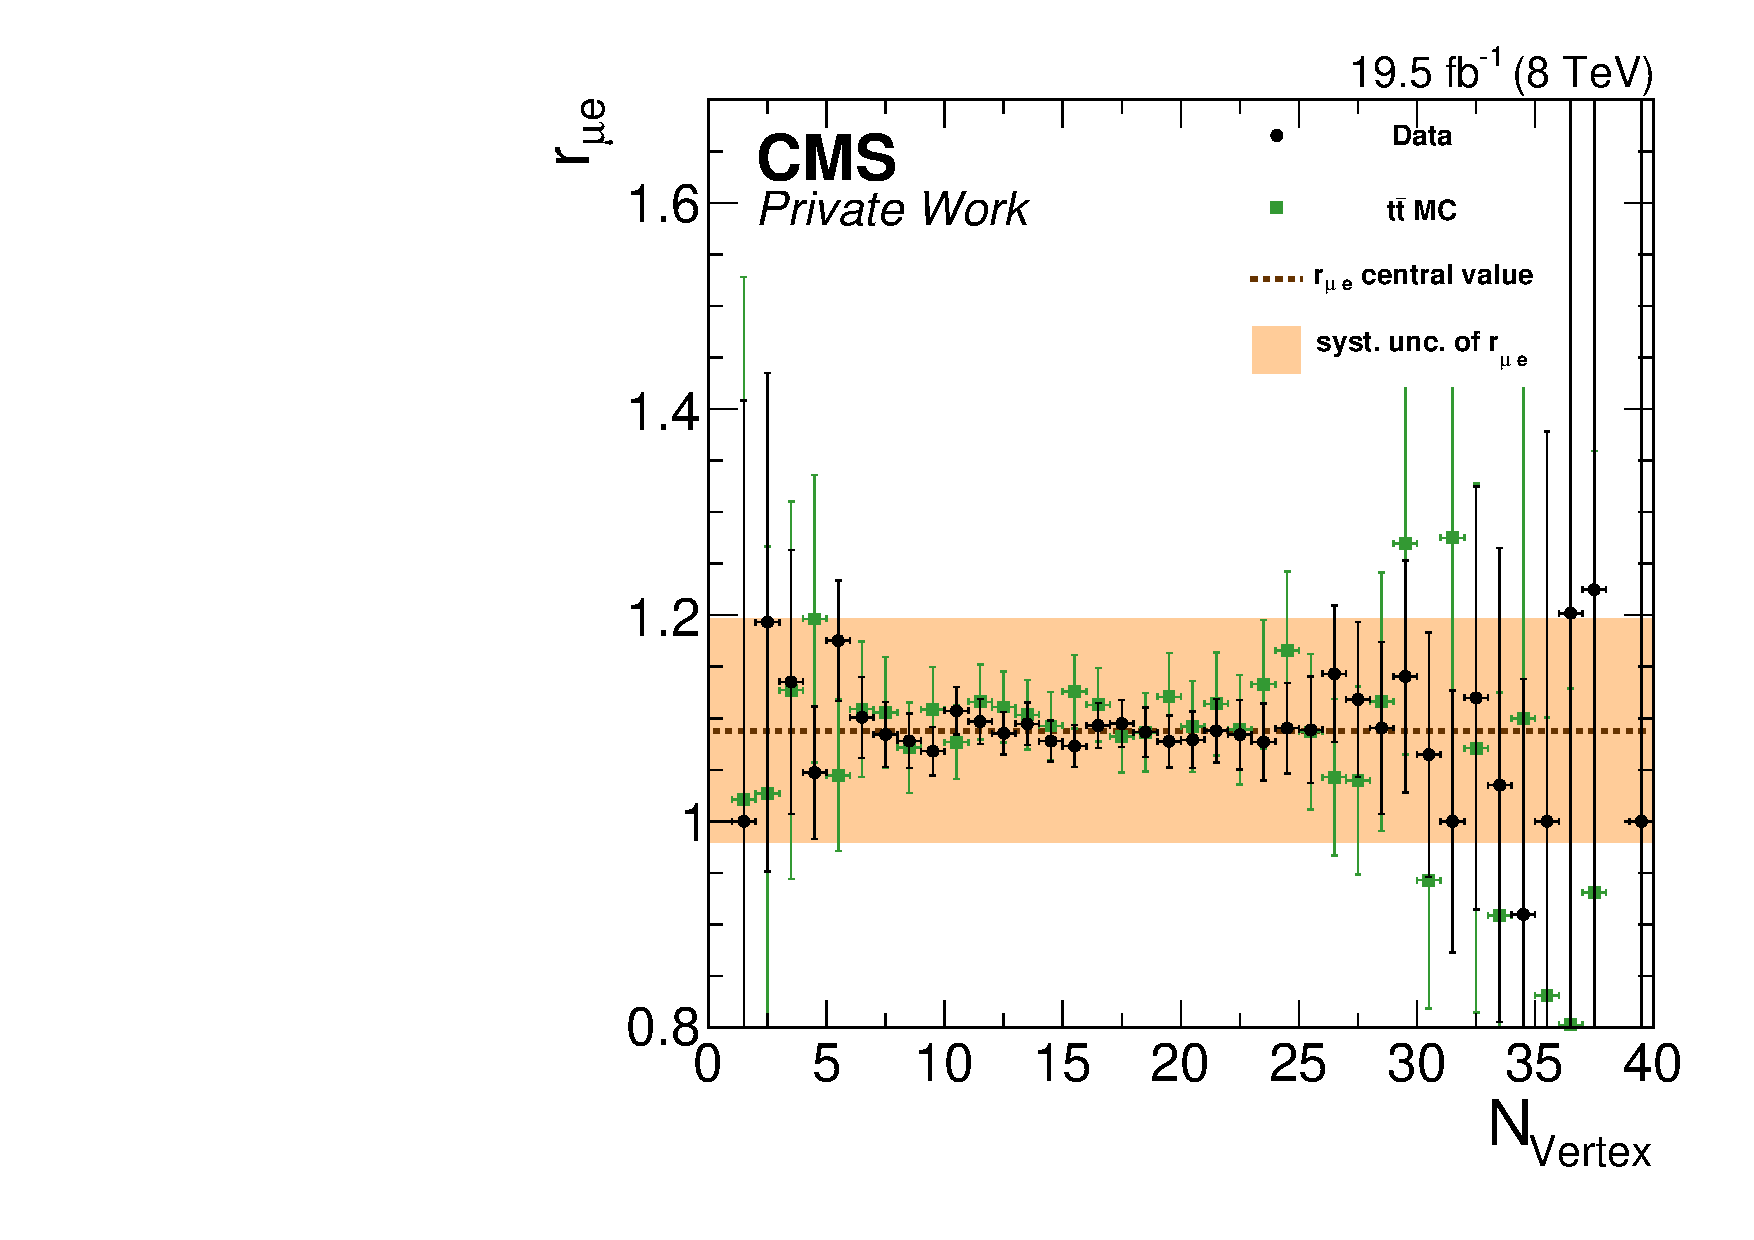
\includegraphics[width=\textwidth]{plots/BG/rmue/rMuE_ZPeakControlCentral_Full2012_nVtx_None.pdf}
\end{minipage}
\begin{minipage}[t]{0.49\textwidth}
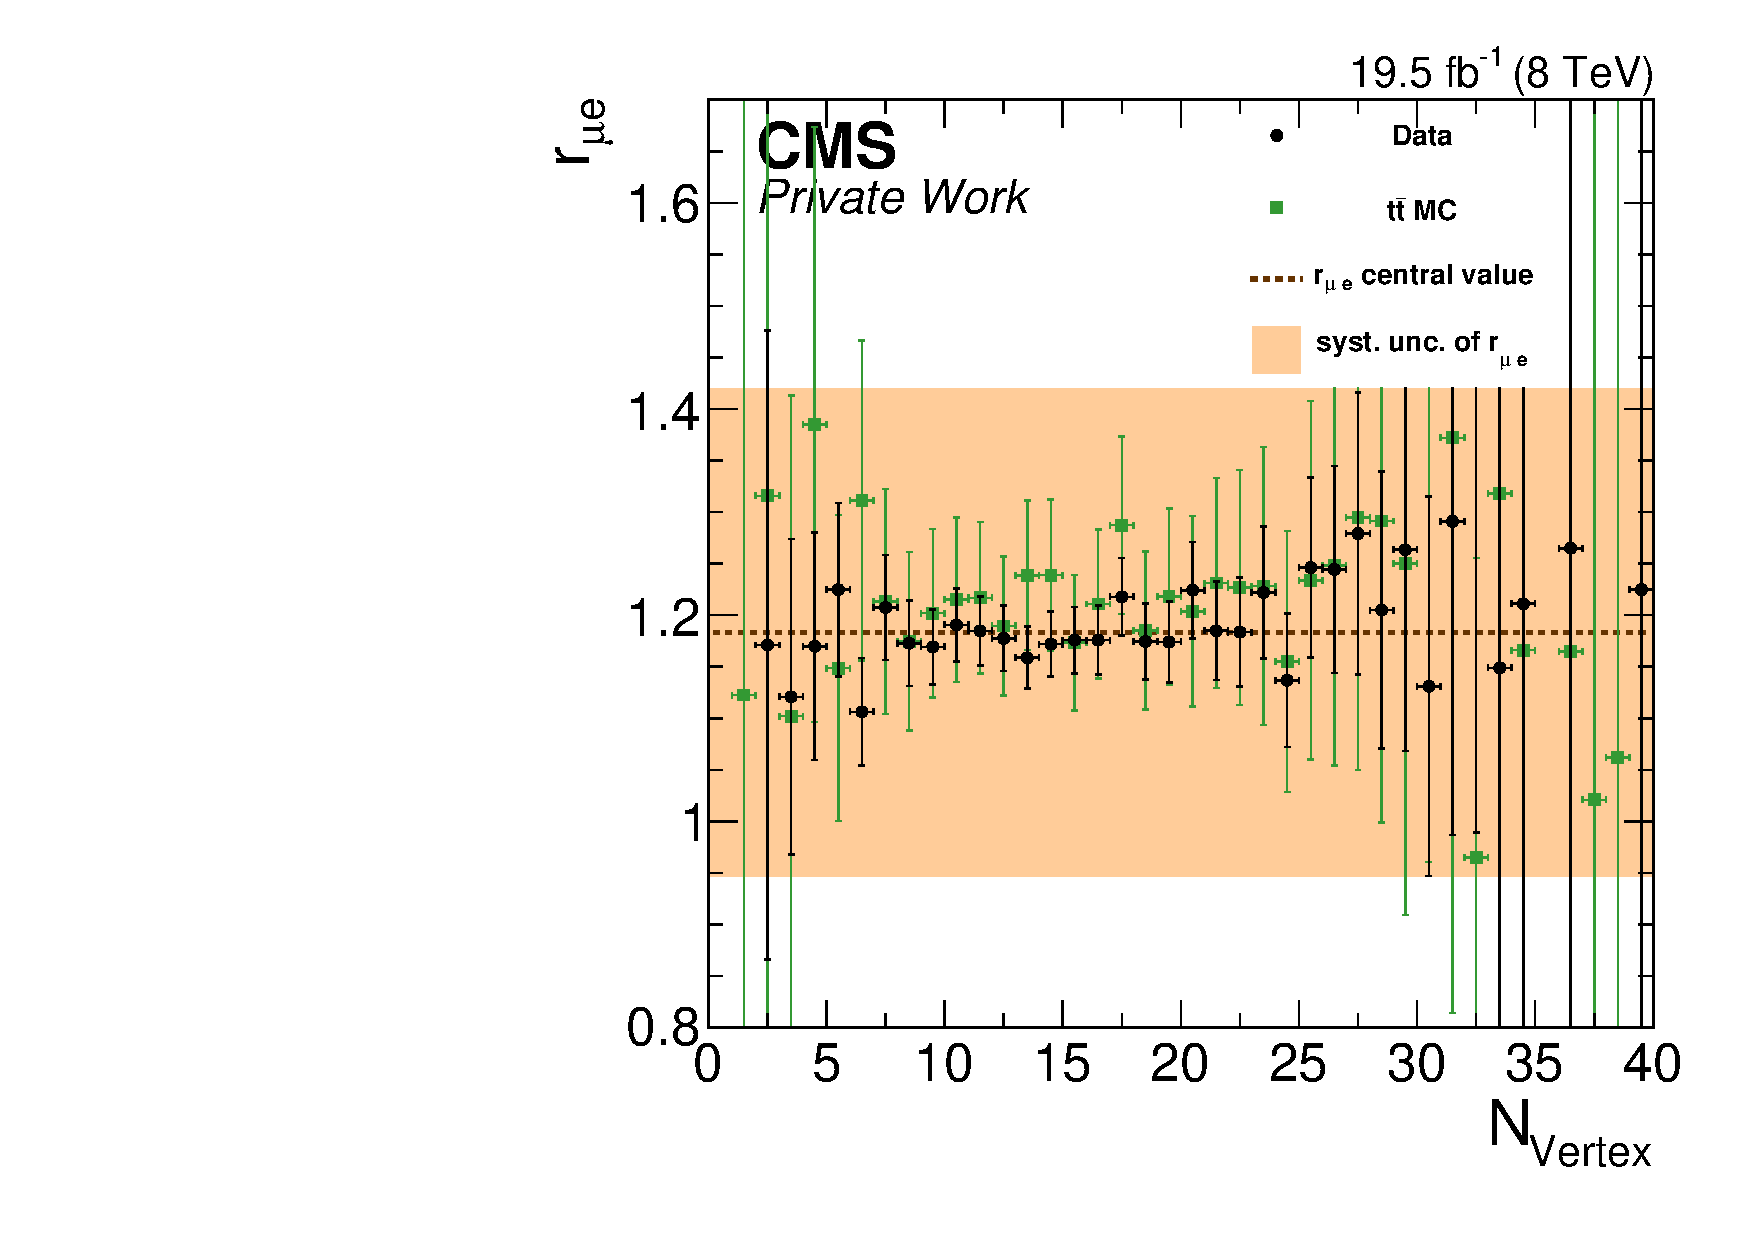
\includegraphics[width=\textwidth]{plots/BG/rmue/rMuE_ZPeakControlForward_Full2012_nVtx_None.pdf}
\end{minipage}
\caption{Dependencies of \rmue on $H_T$ (top) and $N_{vertex}$ (bottom) for the central (left) and forward (right) lepton selection. The results on data are shown in black while $t\bar{t}$ simulation is shown in green. The central value is shown as a brown dashed line while the systematic uncertainty is shown as an orange band.}
\label{fig:rmueDependenciesApp2}
\end{figure} 
